%% Incluindo os pacotes necessários
\documentclass[12pt, a4paper]{article}
\usepackage[utf8]{inputenc}
\usepackage[portuguese]{babel}
\usepackage{booktabs}
\usepackage{titlesec}
\usepackage{titling}
\usepackage{enumitem}
\usepackage{indentfirst}
\usepackage{graphicx}
\graphicspath{{images/}}
\usepackage{fancyhdr}
\usepackage{color}
\usepackage{fancyhdr}
\usepackage{colortbl}
\usepackage{framed}
\usepackage{multicol}
\usepackage{pdfpages} 

%% Definindo o Autor e o título
\author{Victor Emanuel Almeida \and Levi Cícero Arcanjo}
\title{Simulação e algorítimos de semáforo, para o problema ``Leitores e escritores''}

%% Estilo da página
\pagestyle{fancy}
\fancyhead[L]{Item 3~-~Projeto I}
\fancyhead[C]{}
\fancyhead[R]{Sistemas Operacionais}
\fancyfoot[L]{Outubro~-~2020}
\fancyfoot[C]{}
\fancyfoot[R]{-~\thepage~-}
\renewcommand{\headrulewidth}{0.7pt}
\renewcommand{\footrulewidth}{0.3pt}

\titleformat{\section}
{\Large\bfseries}
{\thesection}
{.5cm}
{}

\pretitle{\vfill\begin{center}\LARGE}
\postdate{\end{center}\vfill}

\begin{document}
\begin{titlepage}
\maketitle\thispagestyle{empty}
\end{titlepage}

\section{Algorítimo}

Segue abaixo a implementação de um algorítimo para a resolução:

\begin{figure}[!htb]
	\centering
	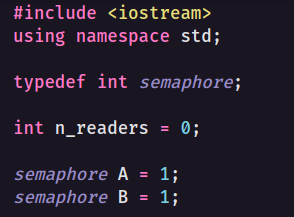
\includegraphics[keepaspectratio]{1.png}
	\caption{\label{fig:1.png} Criação das variáveis e inicializações}
\end{figure}

Nesse primeiro trecho de código, temos a criação e inicialização das variá-~veis, tanto a variável que armazena o número de leitores ativos, quanto os semáforos A e B, que tem função de proteger a variável ``n\underline{ }readers'' e impedir a escrita enquanto alguém estiver lendo ou escrevendo respectivamente.\\

\begin{figure}[!htb]
	\centering
	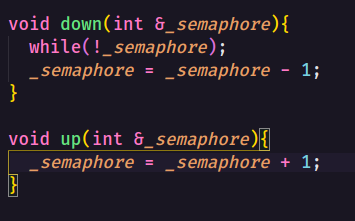
\includegraphics[keepaspectratio, scale=.83]{2.png}
	\caption{\label{fig:2.png} Implementação das funções up e down}
\end{figure}

\begin{itemize}
	\item Função down: Mantém o processo em uma espera ocupada enquanto a variável do semáforo é igual a zero, caso contrário a decrementa.
	\item Função up: incrementa o valor do semáforo caso seja possível.
\end{itemize}

\begin{figure}[!htb]
	\centering
	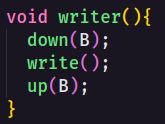
\includegraphics[keepaspectratio, scale=1.2]{3.png}
	\caption{\label{fig:3.png} Implementação do escritor}
\end{figure}

Como podemos ver na figura acima o escritor espera até ser possível realizar o down(), quando concluído ele pode realizar a escrita, pois não existe nenhum outro processo lendo nem escrevendo.\\
\begin{figure}[!htb]
	\centering
	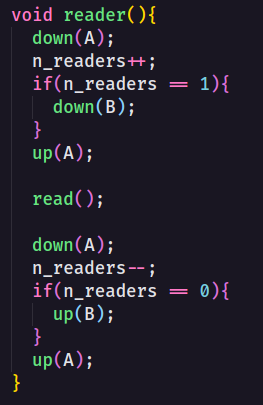
\includegraphics[keepaspectratio, scale=0.98]{4.png}
	\caption{\label{fig:4.png}Implementação do leitor}
\end{figure}

Por fim temos a implementação do leitor, o qual utiliza dois semáforos, sendo o A para modificar a variável ``n\underline{ }readers'', e o B para leitura.

\section{Simulação}

Agora vamos realizar a simulação do algorítimo supracitado, com os seguintes dados:

\begin{multicols}{2}
\begin{itemize}
\footnotesize
	\item Tempo de criação:
	\begin{itemize}
			\item leitor 1 = momento 10
			\item leitor 2 = momento 4
			\item leitor 3 = momento 1
			\item escritor 1 = momento 14
			\item escritor 2 = momento 9
	\end{itemize}
	\item Tempo de execução:
		\begin{itemize}
			\item leitor 1 = momento 8
			\item leitor 2 = momento 7
			\item leitor 3 = momento 15
			\item escritor 1 = momento 6
			\item escritor 2 = momento 5
		\end{itemize}
\end{itemize}
\end{multicols}

%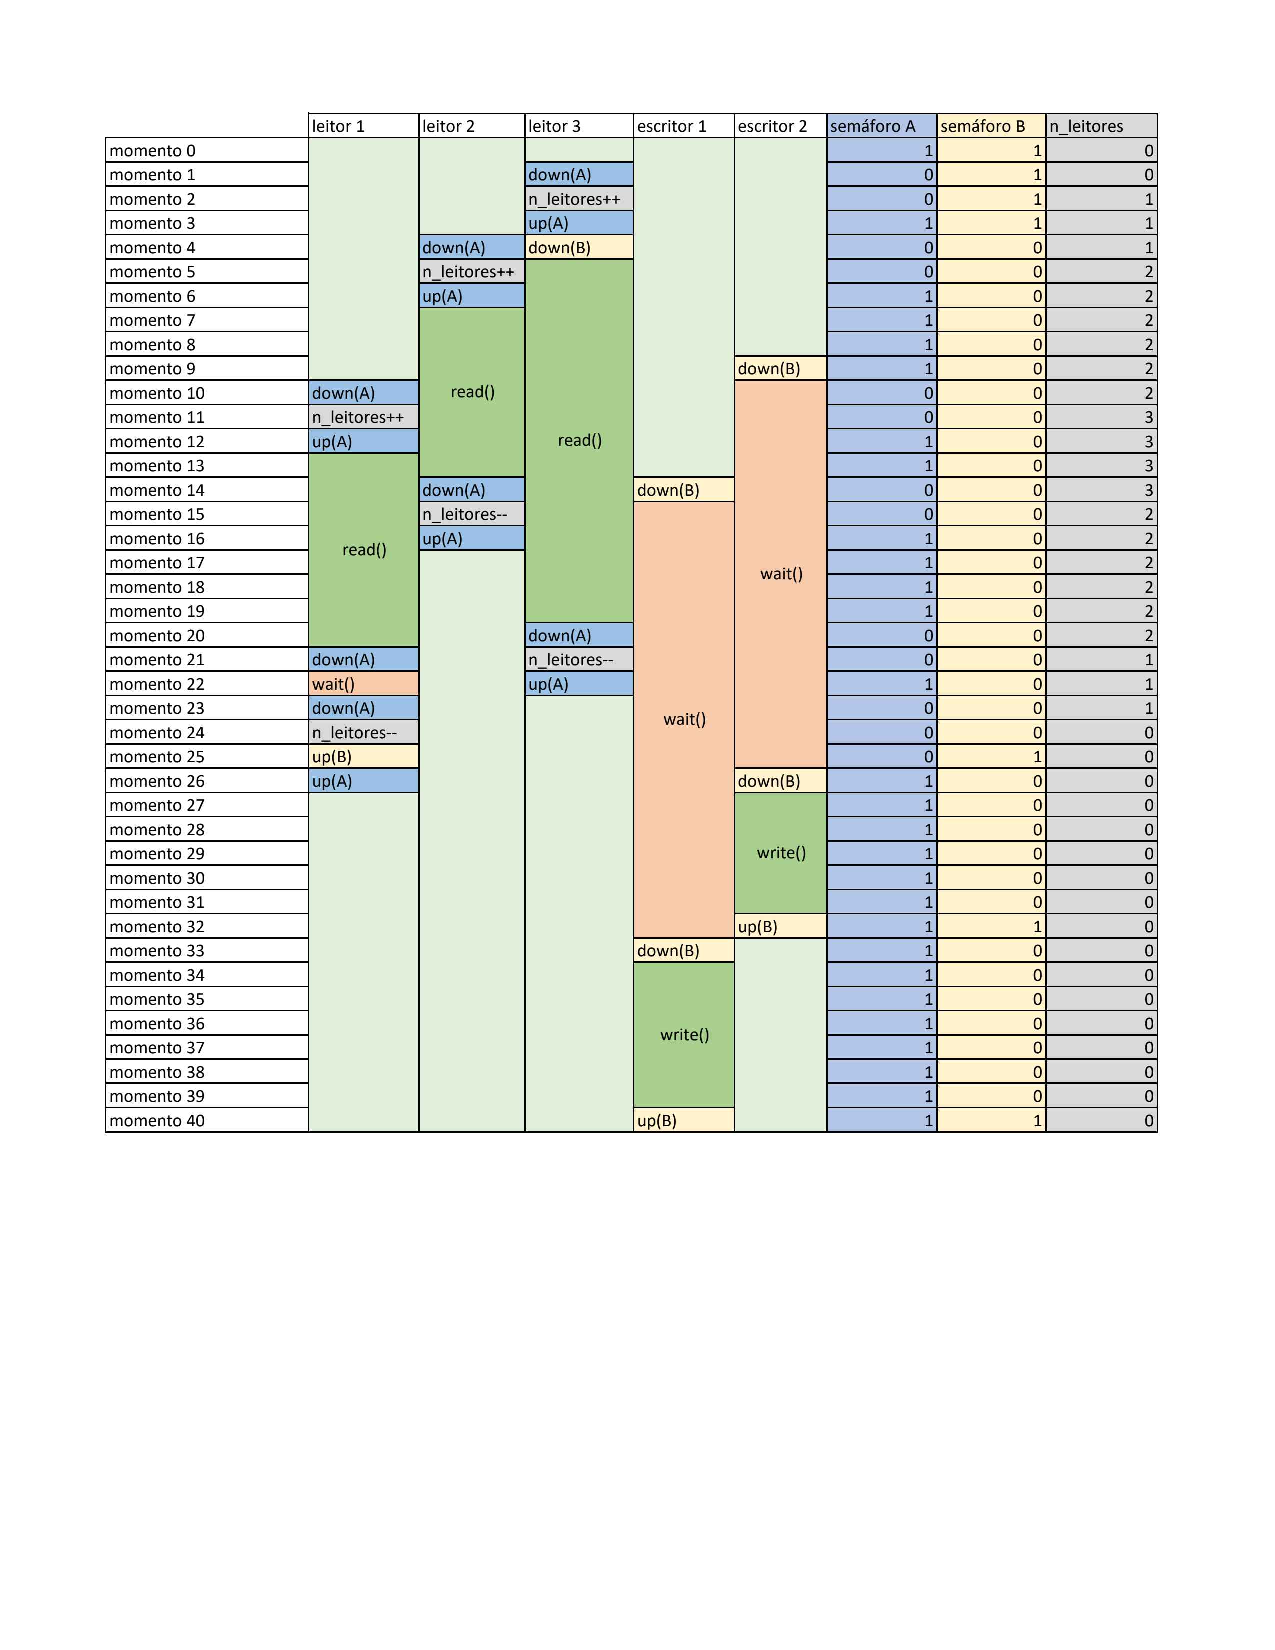
\includepdf[page={1}]{simulation}

%\begin{figure*}[!htb]
%	\centering
%	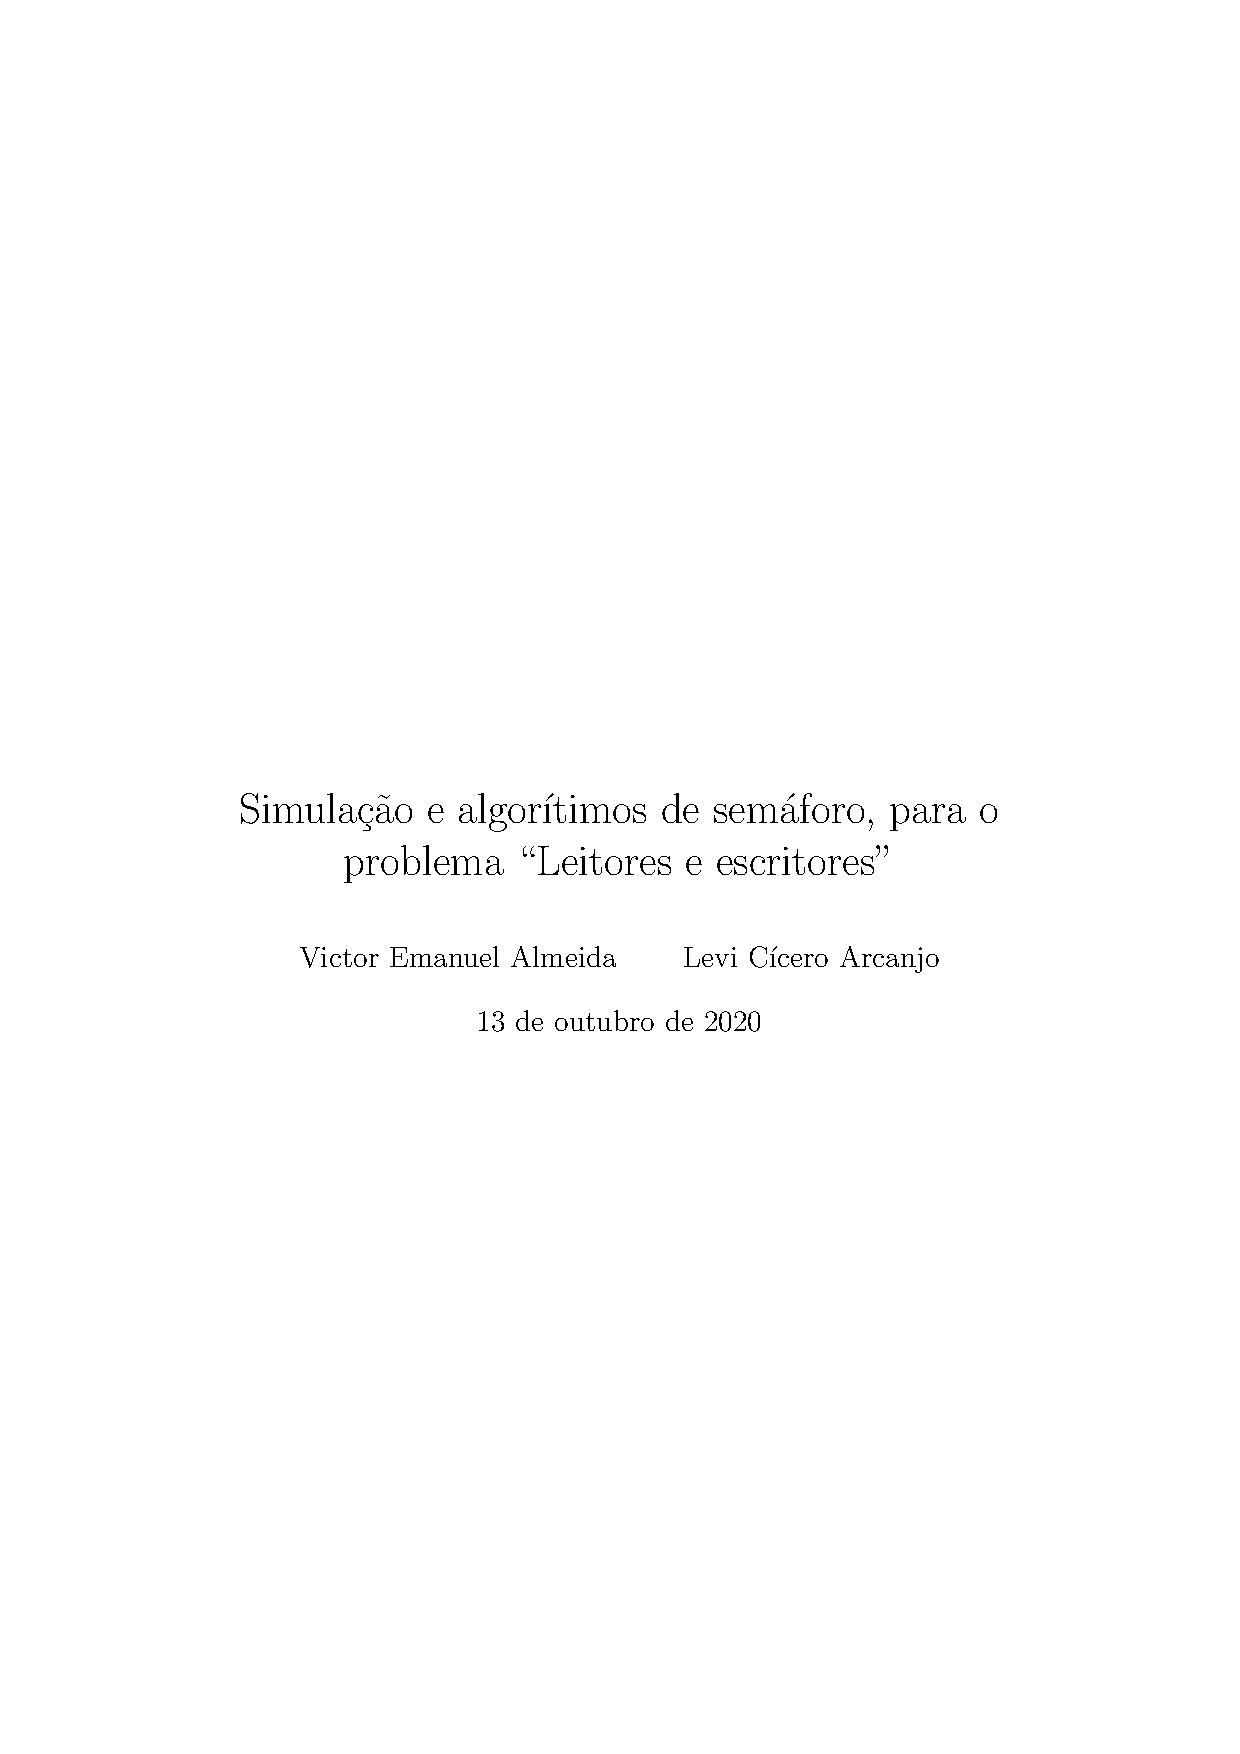
\includegraphics[keepaspectratio, width=.97\textwidth]{tabela.pdf}
%	\caption{\label{fig:tabela.pdf} Simulação do algorítimo}
%\end{figure*}

%\begin{figure}[!htb]
	%\centering
	%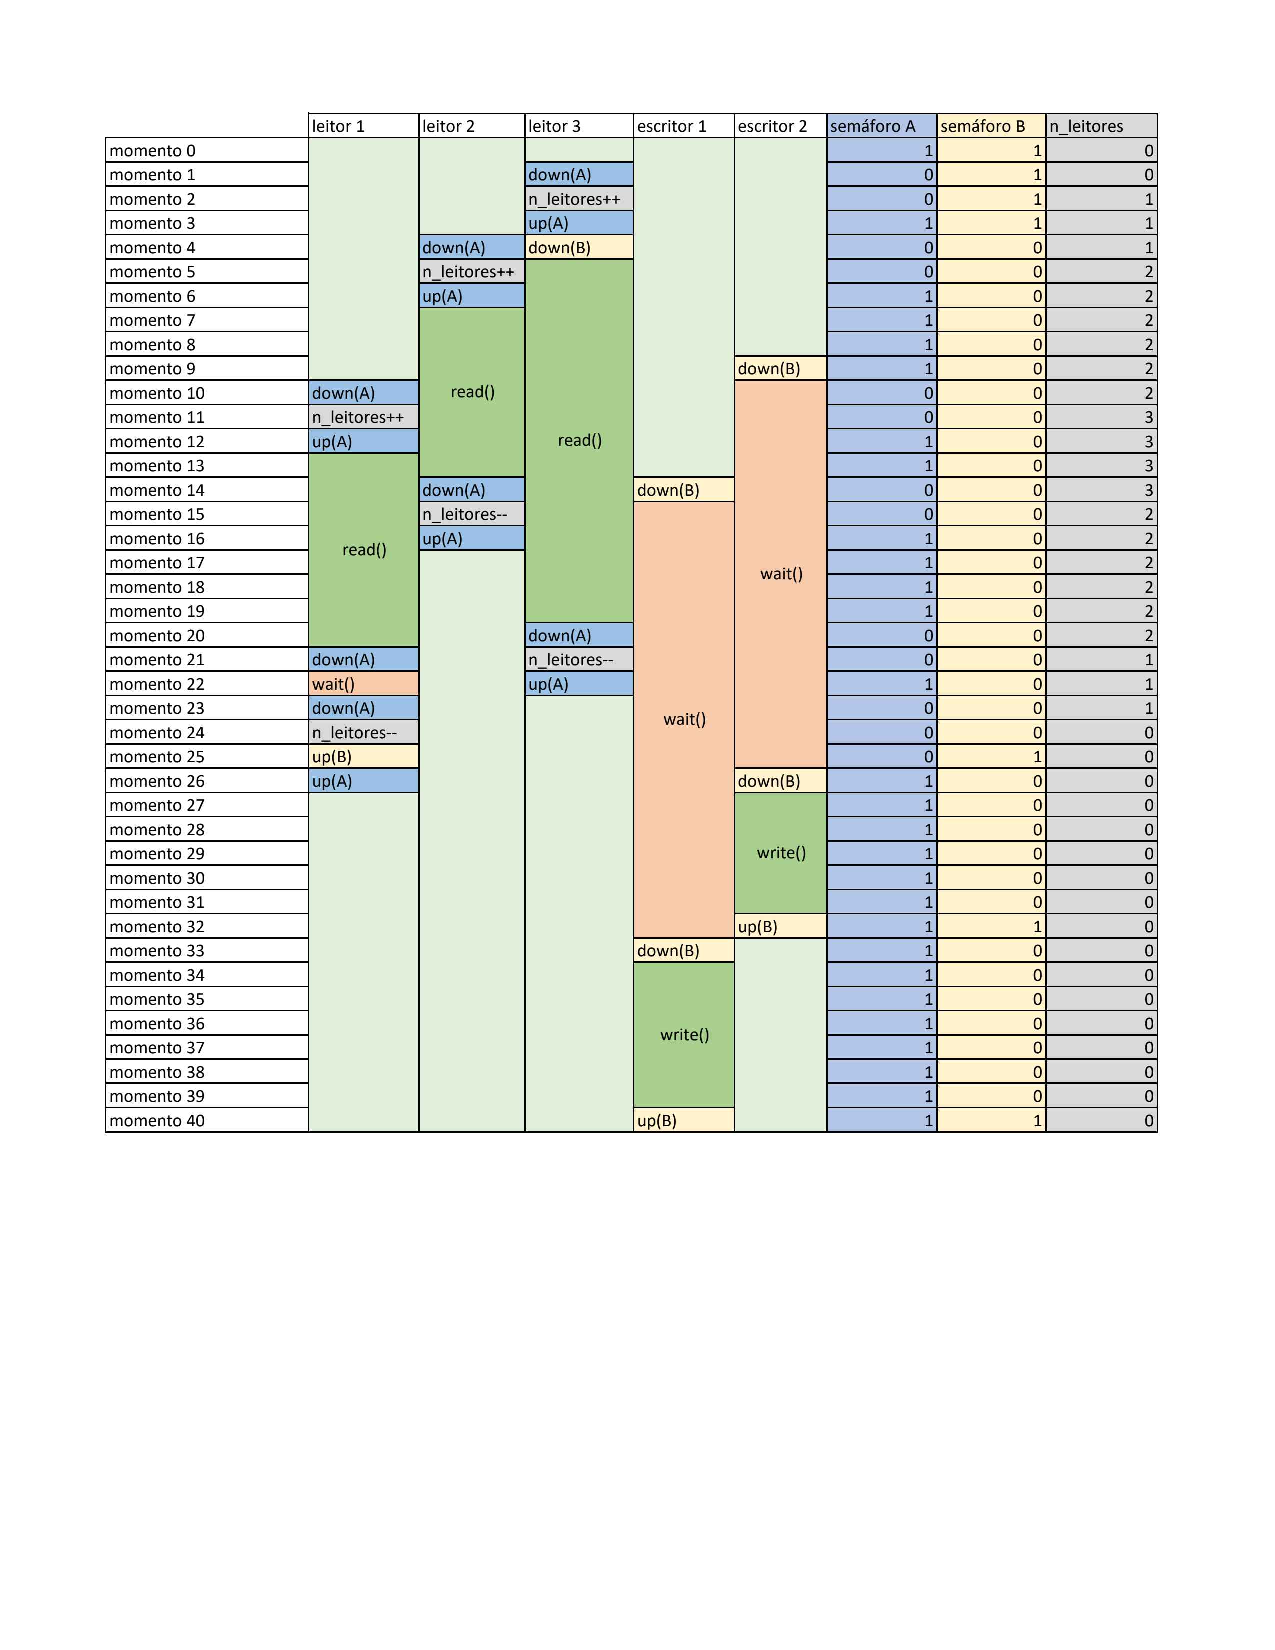
\includegraphics[page=1, scale=.5]{simulation}
	%\caption{\label{fig:}}
%\end{figure}

\begin{figure}[!htb]
	\centering
	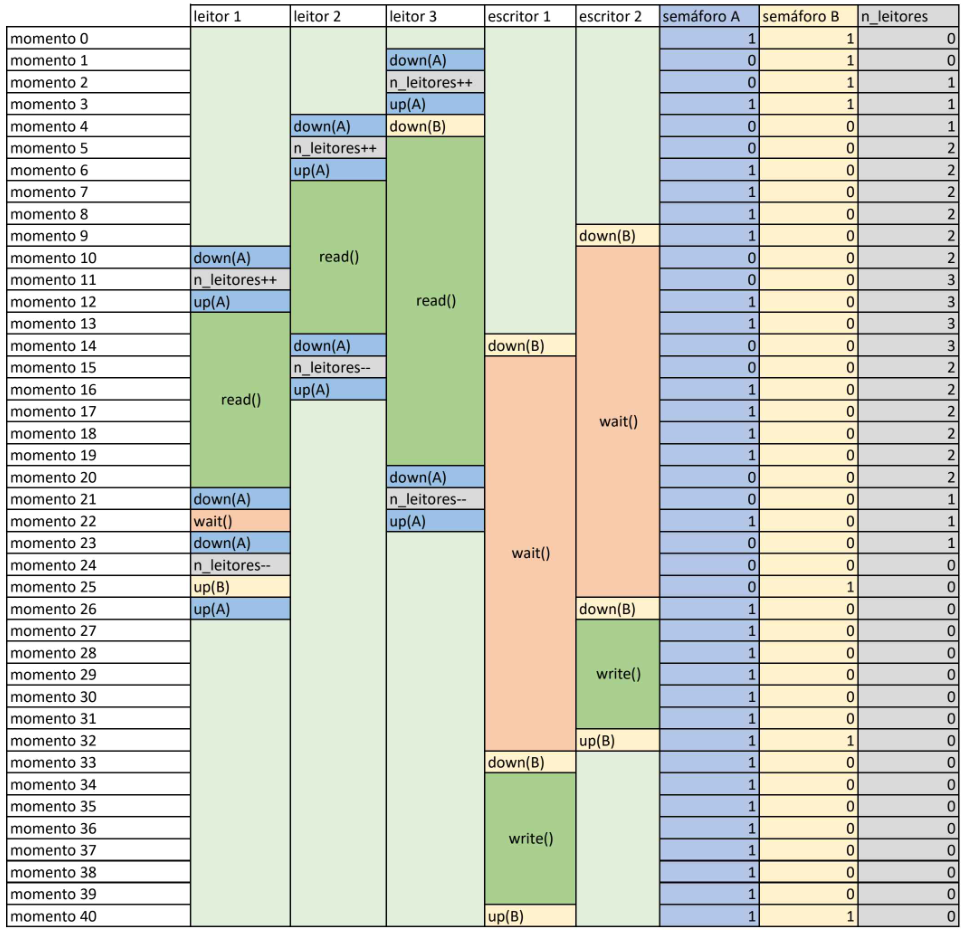
\includegraphics[keepaspectratio,scale=.5]{silulation.png}
	\caption{\label{fig:silulation.png}Simulação do algorítimo}
\end{figure}

\end{document}
